\documentclass[11pt,a4paper]{article}
\usepackage[margin=2.5cm]{geometry}
\usepackage[T1]{fontenc}
\usepackage{amsmath,amssymb,booktabs,graphicx,tabularx,array}
\usepackage[authoryear,round]{natbib}
\usepackage{xurl}
\usepackage[colorlinks=true,linkcolor=blue,citecolor=blue,urlcolor=blue]{hyperref}
\graphicspath{{results/}}
\newcommand{\NationalRows}{13652}
\newcommand{\CountryIDs}{236}
\newcommand{\AccountPass}{183}
\newcommand{\AccountFail}{53}
\newcommand{\PilotPass}{8}

\emergencystretch=3em
\title{Ecological assets behind improving accounts:\\a boundary-matched test of composition masking}
\author{Amin Abaee\\\small Independent Researcher, Tehran, Iran\\\small\href{mailto:amin_abaee@ut.ac.ir}{amin\_abaee@ut.ac.ir}}
\date{}
\begin{document}
\maketitle
\begin{abstract}
Biocapacity accounts and physical ecological assets describe distinct quantities, so agreement between their changes depends on observation boundaries, measurement definitions and uncertainty. This study specifies a forest-led design for comparing national biocapacity with forest extent and above-ground woody biomass, and assesses the suitability of available account and biomass products. The national account workbook contains \NationalRows\ records across \CountryIDs\ country and territory identifiers; \AccountPass\ identifiers satisfy publication, completeness and numerical-consistency criteria for 2015--2023. All eight countries selected for methodological evaluation satisfy these account criteria. Physical comparability requires separate assessment of territorial coverage, forest definitions, missing observations and change uncertainty. Examination of biomass product metadata and methods identifies three consequential distinctions: geographic cells are not equal-area observations, aggregated biomass density is expressed per grid-cell rather than forest area, and change-quality classifications are derived from the same endpoint estimates they assess. The design separates extent and density contributions, quantifies spatially offsetting local net changes, and requires reporting comparisons on identical observational support. The results concern account availability and measurement compatibility; forest-stock trends, account--asset divergence and conversion associations are not estimated. These distinctions define the evidence required for a physical interpretation of changes in biological-supply accounts.
\end{abstract}

\section{Introduction}
Biocapacity is expressed in global hectares, combining physical area with productivity-based factors. Above-ground biomass is a mass of specified living woody material within a geographic support. These quantities are related through ecological production but are not interchangeable measures of ecosystem assets. The distinction between natural-capital stocks and accounting flows has an established basis in the Ecological Footprint literature \citep{Mancini2017}. A quantitative assessment requires separate observation operators and an explicit treatment of their domains.

Composition-dependent land-use models show that transfers towards a land class with a higher annual contribution per hectare can increase a model account while reducing another land class's area \citep{Abaee2026}. Such a mechanism motivates an empirical comparison but does not determine the sign of an observed forest-stock trend. Existing European forest-condition accounting also demonstrates the importance of spatially heterogeneous changes within an aggregate \citep{Maes2023}. Forest condition, extent, biomass and regeneration remain distinct ecological attributes.

The empirical comparison addresses four questions:
\begin{enumerate}
\item How do independently estimated forest extent and above-ground woody biomass change on matched geographic and temporal supports?
\item When national biocapacity increases, do those physical assets increase, decrease or remain unresolved, and how much local change is offset within national totals?
\item Is account--asset divergence associated with independently observed forest-to-cropland conversion after distinguishing harvest, fire, plantation dynamics and regrowth?
\item Does adding independent asset information change an assessment when cases, weights, uncertainty and coverage are held comparable?
\end{enumerate}
The first question establishes the physical outcomes on which the remaining comparisons depend. The sample includes all directions of account and asset change rather than only increasing-account cases. The analysis reported here establishes account availability and measurement definitions; it does not estimate country-level physical changes or conversion associations.

\section{Materials and methods}
\subsection{Sources and observational domains}
The account source is the National Ecological Footprint and Biocapacity Accounts, Edition 2026, results and metadata version 1.0 \citep{Lo2026}. The primary comparison interval is 2015--2023. The secondary comparison domain is 2010--2020, conditional on compatible endpoints and separately justified cross-sensor change uncertainty. Absolute total biocapacity is the principal account measure. Terrestrial, excluding-built-up and forest-component accounts, together with separately labelled per-person values, define alternative account domains. The account's own area fields belong to its input lineage and are not independent physical validation measurements.

The biomass source is ESA Climate Change Initiative Biomass version 7.0 \citep{SantoroCartus2026}. The product provides above-ground woody biomass density estimates for 2005--2012 and 2015--2024. Metadata and coordinate inspection used the nominal 50 km aggregate and the 2010--2020 change product. Scientific interpretation additionally used the Product User Guide and the published change-processing implementation \citep{PUG2026}. Biomass pixel values and national biomass changes were not analysed. The 2010--2020 example describes product structure; it is not a change-validation dataset for the primary interval.

Eight countries were selected for evaluation of geographic and measurement compatibility: Brazil, Indonesia, Democratic Republic of the Congo, Cameroon, Canada, Finland, France and Australia. This purposive selection provides environmental and logistical contrasts rather than a probability sample. Country-level account availability and physical observation compatibility are assessed separately. The full set of account identifiers is retained in the availability analysis, irrespective of any expected direction of ecological change.

\subsection{Account availability and numerical consistency}
Account availability requires a record for every year in 2015--2023, publication flags that permit the relevant biocapacity quantities, and finite, nonnegative required values. Population must be positive. Required fields comprise the five biocapacity components, their total, forest and cropland areas, and population. Flags \texttt{+++}, \texttt{++} and \texttt{+} satisfy the publication criterion; their different trade and consumption detail does not imply a ranking of physical measurement precision. Flags indicating unpublished, missing or estimated-only information do not satisfy the criterion.

The sum of the five published components is compared with the reported total. A tolerance of 3 gha accounts for rounding of five component values and their total. This is a numerical-consistency tolerance, not an ecological threshold. Duplicate country--year keys, missing years and missing required fields are evaluated explicitly. The Supplementary Information specifies the rules and country results.

\subsection{Physical support and stock decomposition}
For a defined support $\Omega$, stock is
\[
Q_t=\int_{\Omega} d_t(x)\,\mathrm dA(x),
\]
where $d_t$ is a biomass density with a specified area denominator. Geographic raster cells require latitude-dependent area weights. The computational method integrates meridian--parallel rectangles on the WGS84 ellipsoid; dateline crossings are divided into separate longitude intervals.

For positive forest areas $A_0,A_1$ and compatible stocks $Q_0,Q_1$, let $D_t=Q_t/A_t$. The symmetric decomposition
\begin{align}
\Delta Q_{\mathrm{extent}}&=(A_1-A_0)(D_1+D_0)/2,\label{eq:extent}\\
\Delta Q_{\mathrm{density}}&=(D_1-D_0)(A_1+A_0)/2\label{eq:density}
\end{align}
sums exactly to $Q_1-Q_0$. The contributions describe changes in aggregate area and mean density; they do not identify causal effects. Zero-area endpoints require a separately defined treatment because forest-only density is undefined there. No physical stock decomposition is estimated from the account area fields alone.

\subsection{Spatially offsetting local changes}
For local stock changes $\Delta Q_i$ on a common observed support, define
\[
G=\sum_i[\Delta Q_i]_+,\qquad L=\sum_i[-\Delta Q_i]_+,
\]
with net change $G-L$, offset mass $\min(G,L)$ and cancellation fraction
\begin{equation}
K=1-\frac{|G-L|}{G+L},\qquad G+L>0.\label{eq:cancel}
\end{equation}
$K$ is undefined when $G+L=0$. The components are positive and negative local net changes, not gross biological growth, recruitment, mortality or harvest. Their values depend on spatial support and measurement error. Interpretation therefore requires effective-resolution and zero-change error-model assessment. Temporal comparisons require repeated observations at identifiable dates rather than interpolated or model-generated annual independence.

\subsection{Uncertainty, validation and information comparisons}
The relevant error structure includes temporal and spatial covariance, systematic bias, land-transition classification error and incomplete coverage. An assessment of biomass levels does not establish the accuracy of biomass change. Independent forest-to-cropland observations require a justified reference design and transition-specific uncertainty \citep{Olofsson2014}.

Reporting comparisons require common cases and weights, together with coverage estimates for the full eligible population and pairwise overlap. Features derived from the target outcomes are distinguished from independently observed information, and algebraically redundant quantities are identified before interpreting an increment in reporting detail. Diagnostic comparisons require separate calibration and held-out evaluation, with uncertainty in estimated error rates. Practical-change thresholds and classification rules must be fixed without using held-out outcomes. Whole-pipeline calibration must account for spatial support, covariance, systematic bias and incomplete coverage, and comparisons with simple account, endpoint and trend baselines must use the same observations. No classification-performance estimates or physical change-resolution thresholds are inferred from the account availability criteria.

\section{Results}
\subsection{Availability of national account data}
The workbook contains \NationalRows\ national records, 51 columns and \CountryIDs\ country or territory identifiers spanning 1961--2025. For 2015--2023, \AccountPass\ identifiers satisfy the account availability criteria and \AccountFail\ do not (Figure~\ref{fig:coverage}). All eight selected countries satisfy these criteria. The maximum discrepancy between the component sum and published total within the interval is 2 gha, within the rounding tolerance. These results describe account coverage rather than a physically matched analytical sample.

\begin{figure}[htbp]
\centering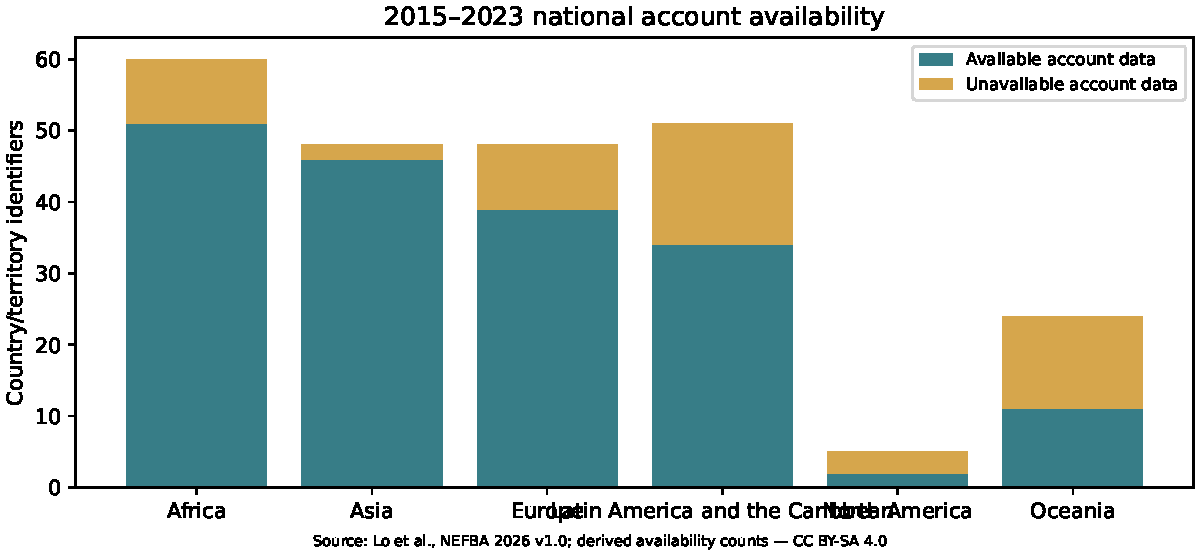
\includegraphics[width=\textwidth]{account_coverage.pdf}
\caption{Availability of national biocapacity account data for 2015--2023 by source UN region. Availability requires complete annual coverage, appropriate publication flags, finite required values and numerical consistency. Data: \citet{Lo2026}; derived availability counts distributed under CC BY-SA 4.0.}\label{fig:coverage}
\end{figure}

\subsection{Biomass support and uncertainty definitions}
The inspected biomass aggregate contains 18 epochs on a $720\times360$ longitude--latitude grid with $0.5^\circ$ spacing. The nominal 50 km designation does not imply equal-area cells. The Product User Guide defines aggregated density per total grid-cell area; it does not define a forest-area-normalized density. Its aggregate uncertainty calculation includes a spatial covariance component \citep{PUG2026}. Consequently, the density denominator, valid-data support and uncertainty interpretation must be specified before a forest stock can be estimated.

The change product includes density difference, change standard deviation and quality-class layers. Quality classes are derived from the endpoint estimates and their uncertainty intervals, with additional growth-limit and spatial-filtering operations. The inspected example calculation of change standard deviation uses the sum of endpoint variances without a temporal covariance term. These classes therefore contain information about the processing rule and its inputs; they are not independent reference observations or calibrated 95\% confidence statements. Supplementary Tables S2--S3 give the source definitions and associated interpretation requirements.

\section{Discussion}
The account coverage supports a multi-country comparison, but availability alone does not establish matched physical support. The distinction is consequential where country definitions, forest masks, mapped observation domains or density denominators differ. Whole-cell biomass averages and forest-only means require different area multipliers. Applying the same multiplier to both would change the physical quantity being estimated.

Spatial compensation also requires measurement-specific interpretation. Opposing local net changes can occur within an increasing national total, but spatial error can produce the same pattern in point estimates. Cancellation must therefore be evaluated with spatial covariance, resolution and zero-change error models. A diagnostic evaluated against a target-derived quality class would measure agreement with that processing rule, rather than independently verified ecological change.

The study is limited to account availability, product definitions and the analytical design. It does not estimate forest-stock trends, account--asset divergence, conversion associations or reporting-rule accuracy. National inference requires territorial and mask reconciliation, independently justified change uncertainty, and coverage-sensitive treatment of missing or converted pixels. Soil, wetlands and fisheries involve different observation domains and are outside the present assessment.

\section{Conclusions}
National biocapacity data for 2015--2023 satisfy the specified availability criteria for \AccountPass\ of \CountryIDs\ country and territory identifiers. Physical account--asset comparison additionally requires aligned boundaries, the correct biomass area denominator, covariance-aware change uncertainty and independent reference information. The extent--density and spatial-cancellation estimands provide explicit quantities for that comparison while preserving distinctions among accounts, stocks, condition and biological flows.

\section*{Data and code availability}
Source datasets are cited in the text. Derived account-availability tables, source definitions, file hashes and computational methods are available at \url{https://github.com/MIKEAA2020/general-sustainability/tree/main/batch%209/agent%202/ecomod_empirical_followup/F03}. NEFBA-derived tables and figures are distributed under CC BY-SA 4.0. Raw biomass files and the Product User Guide are not redistributed.

\section*{Declaration of generative AI in scientific writing}
Arena.ai Agent Mode was used to assist with source-document analysis, computational methods, verification and language editing.

\begin{thebibliography}{9}
\bibitem[Abaee(2026)]{Abaee2026} Abaee, A. (2026). A rising biocapacity total can mask ecological-capital land drawdown: a two-land model. Manuscript. \url{https://github.com/MIKEAA2020/general-sustainability/tree/main/batch%209/agent%202/ecomod_c15}.
\bibitem[Mancini et al.(2017)]{Mancini2017} Mancini, M. S., Galli, A., Niccolucci, V., Lin, D., Hanscom, L., Wackernagel, M., Bastianoni, S., and Marchettini, N. (2017). Stocks and flows of natural capital: Implications for Ecological Footprint. \emph{Ecological Indicators}, 77, 123--128. \url{https://doi.org/10.1016/j.ecolind.2017.01.033}.
\bibitem[Maes et al.(2023)]{Maes2023} Maes, J., Bruz\'on, A. G., Barredo, J. I., Vallecillo, S., Vogt, P., Rivero, I. M., and Santos-Mart\'in, F. (2023). Accounting for forest condition in Europe based on an international statistical standard. \emph{Nature Communications}, 14, 3723. \url{https://doi.org/10.1038/s41467-023-39434-0}.
\bibitem[Olofsson et al.(2014)]{Olofsson2014} Olofsson, P., Foody, G. M., Herold, M., Stehman, S. V., Woodcock, C. E., and Wulder, M. A. (2014). Good practices for estimating area and assessing accuracy of land change. \emph{Remote Sensing of Environment}, 148, 42--57. \url{https://doi.org/10.1016/j.rse.2014.02.015}.
\bibitem[Lo et al.(2026)]{Lo2026} Lo, K., Basnet, N., Miller, E., Srikanthalingam, B., Foley, B., Van Berkum, J. L., Long, A. H., Toneva, P., Ermina, M., and Klinkenberg, C. (2026). \emph{National Ecological Footprint and Biocapacity Accounts, Edition 2026 (1961--2025): Results and metadata, version 1.0}. Footprint Data Foundation. \url{https://footprint.info.yorku.ca/data/}.
\bibitem[Santoro and Cartus(2026)]{SantoroCartus2026} Santoro, M., and Cartus, O. (2026). ESA Biomass Climate Change Initiative: Global datasets of forest above-ground biomass for 2005--2012 and 2015--2024, v7.0. CEDA. \url{https://doi.org/10.5285/6429d1aafe1e43b9b414e4a5a7f8b903}.
\bibitem[CCI Biomass(2026)]{PUG2026} CCI Biomass (2026). \emph{Product User Guide v7.0}. 19 March 2026. \url{https://climate.esa.int/en/projects/biomass/key-documents/}.
\end{thebibliography}
\end{document}
